\documentclass[10pt,a4paper]{article}
\usepackage[latin1]{inputenc}
\usepackage{amsmath}
\usepackage{amsfonts}
\usepackage{amssymb}
\usepackage{graphicx}
\author{Wu Bingzhe\\1200010666\\The school of mathmatical science}
\title{Pattern Recognition Report3\\Chapter3}
\begin{document}
	\maketitle
	\section{Question1}
    In my program of this question,function u1.m compute question(a),u2.m for question(b)
    ,u3.m for question(c),u4.m for question(d).
    \subsection{(a)}
		According to the maximum likelihood estimation on the Gaussian distribution,we can 
		get :
		\begin{equation}
			\hat{\mu}=\dfrac{1}{N}\sigma_{k=1}{N}x_k
		\end{equation}	
		\begin{equation}
			\hat{\Sigma}=\dfrac{1}{N}\Sigma_{k=1}^{N}(x_k-\hat{\mu})(x_k-\hat{\mu})^{T}
		\end{equation}
		In terms of (1) and (2),we could compute the value of the parameters 
		by the program . The results are as follows:
	    \begin{center}
		\begin{tabular}{|c|c|c|}
			\hline  feature& $\hat{\mu}$  & $\hat{\sigma}^2$  \\ 
			\hline  $x_1$& -0.0709 & 0.9062   \\ 
			\hline  $x_2$&  -0.6047& 4.2007  \\ 
			\hline  $x_3$&  -0.9110&  4.5419 \\ 
			\hline 
		\end{tabular} 
		\end{center}	
	\subsection{(b)}
	Similar with (1) and (2),we can get the results as follows:
	
	$\mu_{12}=(-0.0709,-0.6047)^T$ \ $\Sigma_{12}=$
	$\begin{array}{cc}
		0.9062& 0.5678  \\ 
	    0.5678& 4.2007 
	\end{array} 
	$
	
	$\mu_{23}=(-0.6047,-0.9110)^T$ \ $\Sigma_{23}=$
	$\begin{array}{cc}
	4.2007& 0.7337  \\ 
	0.7337& 44.5419 
	\end{array} 
	$
	
	$\mu_{13}=(-0.0709,-0.9110)^T$ \ $\Sigma_{13}=$
	$\begin{array}{cc}
	0.9062& 0.3941  \\ 
	0.3941& 4.5419 
	\end{array} 
	$
	\subsection{(c)}
	According to (1) and (2),we get the results as follows:
	\begin{equation*}
	\mu=(-0.0709,-0.6047,-0.9110)^T
	\end{equation*}
	\begin{equation*}
	\Sigma=\begin{array}{ccc}
	0.9062& 0.5678  & -0.9110  \\ 
	0.5678& 4.2007 & 0.7337  \\ 
	0.3941& 0.7337  &4.5419 
	\end{array} 
	\end{equation*}
	\subsection{(d)}
	The results computed by the program :
	\begin{equation*}
	\mu=(-0.1126,0.4299,0.0037)^T
	\end{equation*}
	\begin{equation*}
	\Sigma=\begin{array}{ccc}
	0.0539& 0  & 0 \\ 
	0& 0.0460  & 0  \\ 
	0& 0 & 0.0073 
	\end{array} 
	\end{equation*}
	\subsection{(e)}
	The value of $\mu_i$ computed by the first three algorithms are the same.
	In terms of that the estimate of $\mu $ is not affected by other dimensional data.So we have the same results .
	
	Similar ,the forth method's results are the same .
	\subsection{(f)}
	According to the forms of (2).The results are the same.
\section{Question2}
In my program ,work3.m calculate the results.And the function $p(x_1,x_2,x_3,h)$ calculate the probability of  the point
 $(x_1,x_2,x_3)$ in three distribution,and decision which class it is.
\subsection{(a)}
When $h=1$The results are:
\begin{center}
\begin{tabular}{|c|c|}
	\hline point & class  \\ 
	\hline $(0.5,1.0,0.0)^T$ & $\omega_2$  \\ 
	\hline  $(0.31,1.51,-0.50)^T$&$\omega_2$  \\ 
	\hline  $(-0.3,0.44,-0.1)^T$&$\omega_2$  \\ 
	\hline 
\end{tabular} 
\end{center}
\subsection{(b)}
When $h=0.1$,the result are same with (a):
\begin{center}
	\begin{tabular}{|c|c|}
		\hline point & class  \\ 
		\hline $(0.5,1.0,0.0)^T$ & $\omega_2$  \\ 
		\hline  $(0.31,1.51,-0.50)^T$&$\omega_2$  \\ 
		\hline  $(-0.3,0.44,-0.1)^T$&$\omega_2$  \\ 
		\hline 
	\end{tabular} 
\end{center}
\section{Question3}
In my program ,function $v1.m$ calculate the one-dimensional density estimation of the n samples.
function $v2.m$ calculate the two-dimensional density estimation of the n samples.function $v3.m$
calculate the probability of the point $(x_1,x_2,x_3)$ 
\subsection{(a)}
Let $k=1$,we get the image :

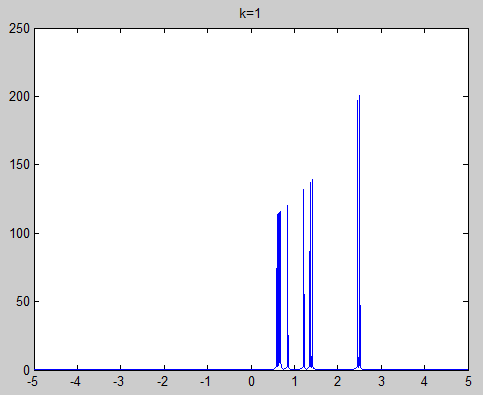
\includegraphics[height=2in,width=4in]{1.png}

Let $k=3$, we get that:

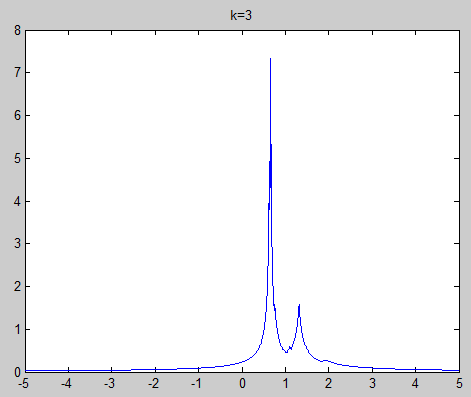
\includegraphics[height=2in,width=4in]{2.png}

Let $k=5$,we get that :

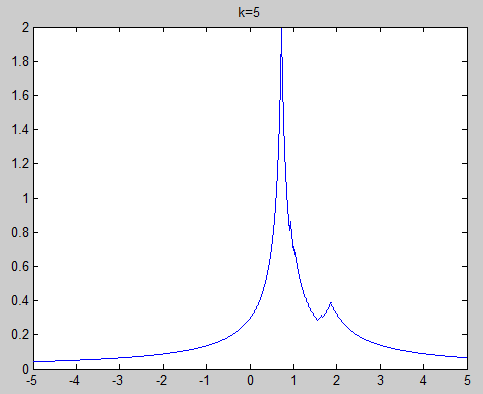
\includegraphics[height=2in,width=4in]{3.png}
\subsection{(b)}
When $k=1$,we have:

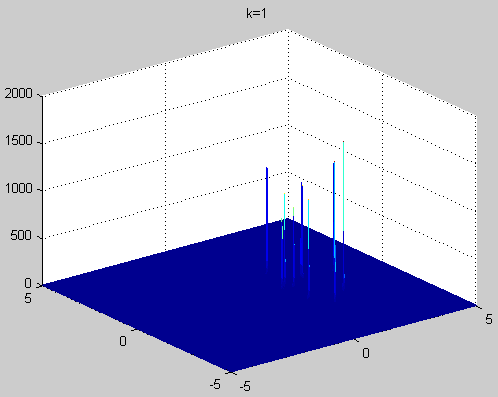
\includegraphics[height=2in,width=4in]{4.png}

When $k=3$,we have :

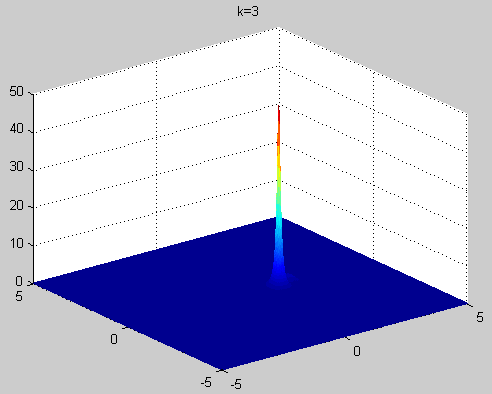
\includegraphics[height=2in,width=4in]{5.png}

When $k=5$,we have:

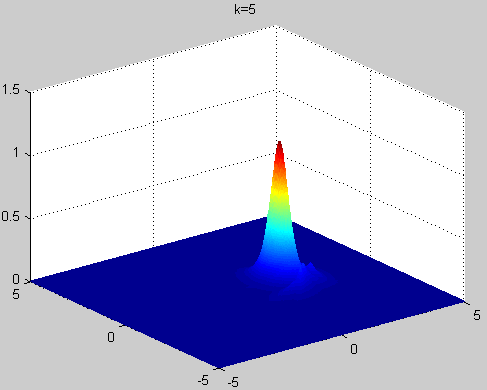
\includegraphics[height=2in,width=4in]{6.png}
\subsection{(c)}
Let $k=3$,we calculate the probability ,the results are follows:
\begin{center}
\begin{tabular}{|c|c|}
	\hline $p_{11}$  & 0.0021  \\ 
	\hline $p_{21}$ & 0.0553 \\ 
	\hline  $p_{31}$ & 0.0358  \\ 
	\hline $p_{12}$ & 0.0043  \\ 
	\hline $p_{22}$ & 9.6478e-04  \\ 
	\hline  $p_{32}$& 0.0021 \\ 
	\hline  $p_{13}$& 0.0026  \\ 
	\hline $p_{23}$ & 0.0869  \\ 
	\hline $p_{33}$  & 0.0085  \\ 
	\hline 
\end{tabular} 
\end{center}
\end{document}
